In Computer Management vind je onder \textquote{System Tools} het kopje \textquote{Local Users and Group}. We zien bij \textbf{Groups} een overzicht van alle aanwezige groepen op ons systeem.

\begin{minipage}[t]{\linewidth}
\raggedright
\adjustbox{valign=t}{%
	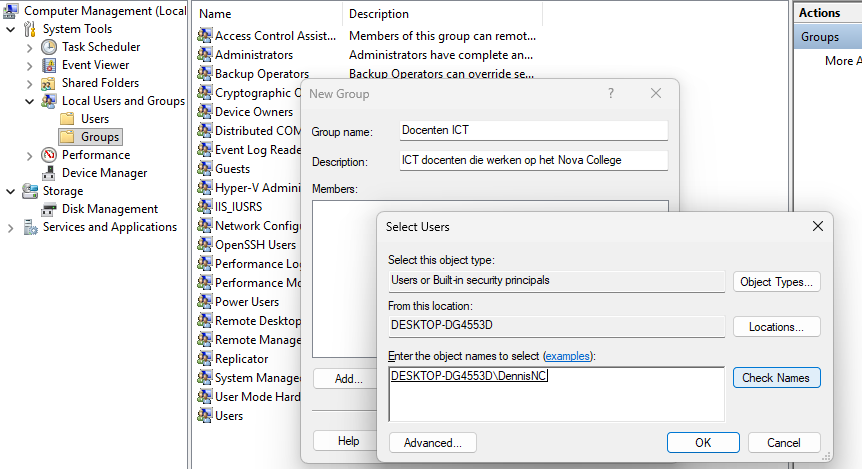
\includegraphics[width=0.99\linewidth]{computer_management-groups_add.png}%
}
\end{minipage}

Na een naam voor de groep en een beschrijving kunnen we gebruikers aan de groep toevoegen. Via \textquote{Object Types} kunnen we kiezen in welke objecten er gezocht moet worden naar de naam die we later op gaan geven. \textquote{Locations} geeft de mogelijkheid om te selecteren vanaf welke machine we de accounts willen halen, voor nu is dat onze eigen machine. Daarna kunnen we opgeven welke gebruikers we willen toevoegen aan onze groep. Als je meer dan 1 gebruiker wil toevoegen dan moeten de verschillende gebruikersnamen gescheiden worden door een punt-komma (;).

Je kan de simpele gebruikersnaam zoals \textquote{DennisNC} opgeven en dan de \textquote{Check Names} knop gebruiken om ze aan te laten vullen met de computernaam. De computer naam is het Domein waarin de gebruikers leven. Je lokale domein is de naam van je computer, je globale domein is het domein (internet domein) waarin je computer is opgenomen (bijvoorbeeld microsoft.com).

We kunnen een gebruiker ook toevoegen aan een bestaande groep. Zo kunnen we een gebruiker lid maken van de groep Administrators om het de rechten van de administrator te geven. Wat op zal vallen is dat een gebruiker dan niet alleen bij de bestanden van de Administrator kan, maar ook alle andere rechten van de Administrator heeft gekregen. Het gaat niet om alleen data maar ook om functionele rechten.

